\ylDisplay{Kujutis läätsega} % Ülesande nimi
{EFO žürii} % Autor
{piirkonnavoor} % Voor
{2017} % Aasta
{P 2} % Ülesande nr.
{3} % Raskustase
{
% Teema: Valgusõpetus
\ifStatement
Konstrueerige ese $AB$, mille kujutis $A'B'$ on antud. 
\begin{center}
	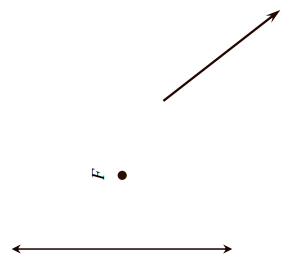
\includegraphics[width=0.5\linewidth]{2017-v2p-02-yl.PNG}
\end{center}
\fi
\ifHint
Esmalt tuleb joonistada risti läätsega tema keskpunkti läbiv optiline peatelg. Seejärel on võimalik "tagurpidi" konstrueerides kujutada eseme asukoht.
\fi
\ifSolution
Joonistame läätse optilise peatelje, mis on risti läätsega ja läbib läätse fookuse, et määrata läätse optiline keskpunkt $O$. Joonistame punktist $A'$ kiire, mis läbib läätse optilise keskpunkti. Joonistame punktist $A'$ kiire, mis läbib läätse fookuse ja pärast läätse on paralleelne optilise peateljega. Kiirte lõikepunkt on eseme punkt $A$. Sama punkti $B'$ korral.
\begin{center}
	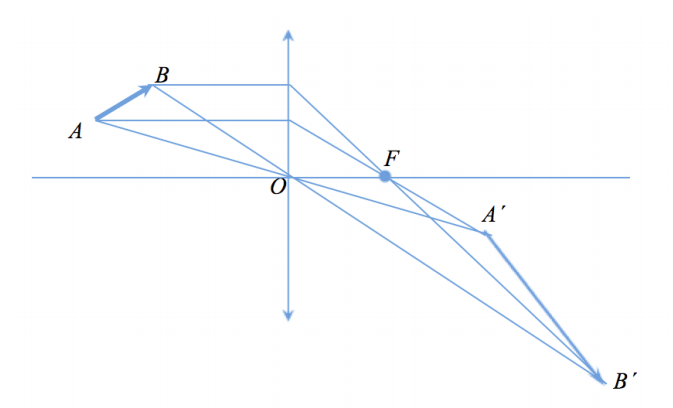
\includegraphics[width=0.5\linewidth]{2017-v2p-02-lah.PNG}
\end{center}
\fi
}
